% ----------------------------  PACKAGES ---------------------------- 
\documentclass[french,a4paper,11pt]{article}
\usepackage[utf8]{inputenc}
\usepackage[T1]{fontenc}
\usepackage[french]{babel}          % Switch french with english
\usepackage{csquotes}
\usepackage{tcolorbox} % Boite de vouleur
\usepackage{amsmath} % Balises de maths
\definecolor{darkblue}{rgb}{0.0, 0.0, 0.4} % Darker shade of blue
\definecolor{darkgreen}{rgb}{0.0, 0.4, 0.0} % Darker shade of blue
\definecolor{darkred}{rgb}{0.4, 0.0, 0.0} % Darker shade of blue
\usepackage[colorlinks=true, linkcolor=darkblue, citecolor=darkgreen, filecolor=purple, urlcolor=darkred]{hyperref}  % \cite, \ref, \cref deviennent clickables
\usepackage[capitalise,noabbrev]{cleveref} 
\usepackage{graphicx}               % For including figures
\usepackage{caption}                % For better control over captions in tables and figures
\usepackage{multicol}
\usepackage{multirow} 
\usepackage{listings}
\usepackage{subfiles}
\usepackage[backend=biber,style=alphabetic,sorting=none]{biblatex}
\usepackage{booktabs} 
\usepackage{array} % Pour définir une colonne d'alignement avec un style particulier
\usepackage[acronym]{glossaries} % nonumberlist pour effacer les numéros
\usepackage{subcaption}
\usepackage{pdflscape}
\usepackage{siunitx} % \num (affichage gros nombre)
\sisetup{group-separator = \ } % Espace insecable pour seppare les chiffres des nombre (5,00,00 devient 5 000 000)
\usepackage{titlesec}
\usepackage{needspace}
\usepackage{enumitem}
\usepackage{chngcntr} % Permet de changer le compteur de figure et de table
\usepackage[toc,page]{appendix}


%\usepackage{helvet}
% \renewcommand{\familydefault}{\sfdefault}
% % Use Adobe Helvetica for math
% \usepackage{sansmath}
% \sansmath
% ------------------------------------------------------------------- 

% ----------------------------  ALLIASES ---------------------------- 
\newcommand{\redbracket}[1]{\textbf{\textcolor{red}{[ #1 ]}}}
\newcommand{\purplebracket}[1]{\textbf{\textcolor{purple}{[ #1 ]}}}
\newcommand{\greenbracket}[1]{\textbf{\textcolor{darkgreen}{[ #1 ]}}}
% -------------------------------------------------------------------


% ----------------------------  CODES ---------------------------- 
\definecolor{codeblue}{rgb}{0.1,0.1,0.7}
\lstset{
    language=bash,                          % The programming language of the code
    basicstyle=\ttfamily\small,             % The style of the code
    keywordstyle=\color{codeblue},          % Keyword style
    commentstyle=\color{green!50!black},    % Comment style
    numbers=left,                           % Line numbers on the left
    numberstyle=\tiny\color{gray},          % Line number style
    stepnumber=1,                           % Line numbers incrementing by 1
    showstringspaces=false,                 % Don't show spaces in strings
    tabsize=4,                              % Tab size
    breaklines=true,                        % Automatic line breaking
    breakatwhitespace=false,                % Automatic breaks at whitespace
    frame=single,                           % Frame around the code
    captionpos=b,                           % Caption position (bottom)
    morekeywords={} % Define size_t as a keyword
}
% ---------------------------------------------------------------- 


% ----------------------------  GEOMETRY ---------------------------- 
\usepackage[top=3cm, bottom=3cm, left=3cm, right=3cm, marginparwidth=2.5cm]{geometry}
% ------------------------------------------------------------------- 


% ----------------------------  SECTIONS ---------------------------- 
% Redéfinir \section
\titleformat{\section}
  {\vspace{1em}\normalfont\Large\bfseries}
  {\thesection}{1em}{}

\titlespacing*{\section}
  {0pt}{\dimexpr\baselineskip}{\dimexpr\baselineskip/2}

% Redéfinir \subsection
\titleformat{\subsection}
  {\vspace{1em}\normalfont\large\bfseries}
  {\thesubsection}{1em}{}

\titlespacing*{\subsection}
  {0pt}{\dimexpr\baselineskip}{\dimexpr\baselineskip/2}

% Redéfinir \subsubsection
\titleformat{\subsubsection}
  {\vspace{1em}\normalfont\normalsize\bfseries}
  {\thesubsubsection}{1em}{}

\titlespacing*{\subsubsection}
  {0pt}{\dimexpr\baselineskip}{\dimexpr\baselineskip/2}
% ------------------------------------------------------------------- 



% ----------------------------  ITEMIZE ---------------------------- 
% Ajouter un saut de ligne après les environnements d'énumération
\setlist[itemize]{after=\vspace{0.5\baselineskip}}
\setlist[enumerate]{after=\vspace{0.5\baselineskip}}
\renewcommand*\descriptionlabel[1]{\hspace\labelsep\texttt{#1}}
\setlist[description]{after=\vspace{0.5\baselineskip}}
% ------------------------------------------------------------------



% ----------------------------  CREF ---------------------------- 
% Redéfinir les noms des types de références en minuscules
\crefname{section}{section}{sections}
\crefname{figure}{figure}{figures}
\crefname{table}{tableau}{tableau}

% Optionnel : Redéfinir les noms avec une majuscule (pour \Cref)
\Crefname{section}{Section}{Sections}
\Crefname{figure}{Figure}{Figures}
\Crefname{table}{Tableau}{Tableau}
% -------------------------------------------------------------- 


% ----------------------------  BIBLIO ---------------------------- 
\addbibresource{ref.bib}
% ----------------------------------------------------------------- 

\selectlanguage{french}

% Début du document
\begin{document}
\title{Analyse de données
transcriptomiques d’espèces sauvages
apparentées au blé}
\author{Florent MARCHAL}
\institute{INRAE - UMR AGAP - Ge2POP}

\subfile{Specials/first_page}

\section{Introduction}

\begin{frame}
    \frametitle{Problématique}
    
    \begin{alertblock}{Objectif}
       Évaluer la qualité des données de séquençage issues d’une étude antérieure (\cite{burgarella_mating_2024}) pour déterminer si celles-ci peuvent être utilisées pour rechercher des traces de sélection.
    \end{alertblock}
    
\end{frame}


\begin{frame}
    \frametitle{Plan}
    
    \tableofcontents[sectionstyle=show, subsectionstyle=show/show/hide]
    
\end{frame}


\subsection{Modèles biologiques}
\begin{frame}

    \frametitle{Modèles biologiques}
    \begin{block}{Espèces utilisées}
        \begin{itemize}
            \item 13 espèces sauvages apparentés au blé 
            \item Famille des \textit{Poaceae} (Graminées)
            \item Phylogénie connue (\cite{burgarella_mating_2024})
        \end{itemize}
    \end{block}
    \pause
    \vspace{0.25cm}
    \begin{block}{\textit{Triticum urartu}}
        \begin{itemize}


            \item Mode de reproduction fortement autogame 
            \item Génome diploide de $4,8Gpb$  ($35,5$ fois plus
grand qu’\textit{Arabidopsis thaliana} ($0, 135Gpb$))
            \item Partie « A » du génome du blé tendre (Froment)
            \item Génome de référence disponible
        \end{itemize}
    \end{block}
\end{frame}

\subsection{Données}
\begin{frame}
    \frametitle{Données}
    \begin{block}{Données brutes}
        \begin{itemize}
            \item Fichier FASTQ
            \item 44 fichier de \num{24 000 000} reads
            
        \end{itemize}
    \end{block}

    \pause
    
    \begin{block}{Reférenes}
        \begin{itemize}
            \item Genone de référence
            \item Transcriptome de référence
            \item Ancien transcriptome de référence (ex-nihilo)
            
        \end{itemize}
    \end{block}

    \pause
    
    \begin{block}{Données raffinés}
        \begin{itemize}
            \item Fichier BAMS
            \item Tableaux fait avec "dNdSpiNpiS" \cite{dNdSpNpS}
        \end{itemize}
    \end{block}
\end{frame}


\section{Vocabulaire}
\begin{frame}
	\tableofcontents[sectionstyle=show/shaded,subsectionstyle=show/show/hide,subsubsectionstyle=show/show/hide]
\end{frame}

\subsection{Synonyme et non synonyme}
\begin{frame}
    \frametitle{Synonyme et non synonyme}
    \subfile{Tabs/seq-A-Presentation}

    \pause
    \small
    \begin{itemize}
        \item \textbf{Sites synonyme}
        \item \textbf{Sites non synonyme}
    \end{itemize}

\end{frame}





\begin{frame}
    \frametitle{Synonyme et non synonyme}
    \subfile{Tabs/seq-B-Synonime}
    \small

    \begin{itemize}
        \item \textbf{Sites synonyme} codons codants pour un même acide aminé
        \item \textbf{Sites non synonyme} 
    \end{itemize}


\end{frame}


\begin{frame}
    \frametitle{Synonyme et non synonyme}
    \subfile{Tabs/seq-C-NonSynonime}
    \small
    \begin{itemize}
        \item \textbf{Sites synonyme} codons codants pour un même acide aminé
        \item \textbf{Sites non synonyme} codons ne codants pas pour un même acide aminé
    \end{itemize}

\end{frame}

\subsection{Polymorphisme et substitutions}
\begin{frame}
    \frametitle{Polymorphisme et substitutions}
   
    \begin{block}{Les sites synonymes peuvent s'étudiés :}
        \begin{description}
            \item [au sein d’une même population :] on parle de polymorphisme
            \item [au sein d’un groupe de population :] on parle de substitutions 
        \end{description}
    \end{block}
    


\end{frame}

\subsection{Substitutions}
\begin{frame}
    \subfile{Tabs/seq-D-Substitution.tex}

\end{frame}

\section{Théorie}
\begin{frame}
	\tableofcontents[sectionstyle=show/shaded,subsectionstyle=show/show/hide,subsubsectionstyle=show/show/hide]
\end{frame}

\subsection{Sélections}
\begin{frame}{Sélections}
	\begin{block}{Absence de sélection}
        \begin{itemize}
            \item Les sites évoluent à la même vitesse.
        \end{itemize}
    \end{block}

 
    \pause
    \begin{block}{Sélection purificatrice}
        \begin{itemize}
            \item S'oppose aux mutations non synonymes
            \item Conserve les séquences
        \end{itemize}
    \end{block}

    \pause
    \begin{block}{Sélection positive}
        \begin{itemize}
            \item Favorise la fixation de mutations non synonymes
        \end{itemize}
    \end{block}
    
\end{frame}

\subsection{Indicateurs}
\begin{frame}
    \frametitle{Indicateurs}
    
    \begin{table}
        \centering
        \small
        \begin{tabular}{c c c}
           
            \toprule
              & Site Fixés & Sites polymorphique \\
            \midrule
            Non synonyme & $D_n$ & $P_n$ \\
            Synonyme & $D_s$ & $P_s$ \\

            \bottomrule
           
        \end{tabular}
         \caption{Indicateurs utilisés pour la recherche de traces de sélections}
    \end{table}

    \begin{exampleblock}{Utilisation}
        \begin{itemize}
            \item  $\frac{P_n}{P_s}$ Étude du polymorphisme 
            \item  $\frac{D_n}{D_s}$ Étude des substitutions
            \begin{itemize}
                \item $\frac{D_n}{D_s} > 1$ Conservation de la substitution
                \item $\frac{D_n}{D_s} < 1$ Élimination de la substitution
            \end{itemize}

        \end{itemize}
    \end{exampleblock}

    
\end{frame}

\begin{frame}
    \frametitle{Conclusion}
     \begin{alertblock}{ Besoin de sites variables}
        \begin{itemize}
            \item[$\rightarrow$] Suffisamment de sites
            \item[$\rightarrow$] Suffisamment grand nombre de séquence
        \end{itemize}
    \end{alertblock}
    
\end{frame}

\section{Quantification des SNP}
\begin{frame}
	\tableofcontents[sectionstyle=show/shaded,subsectionstyle=show/show/hide,subsubsectionstyle=show/show/hide]
\end{frame}

\subsection{Outil fait maison}
\begin{frame}{Création d'un outil}
    \begin{block}{Données de initiales}
        \begin{itemize}
            \item Nombre de SNP par contig
        \end{itemize}
    \end{block}

    \begin{block}{Definitions}
        \begin{itemize}
            \item SNP : \textit{Single nucléotidique polymorphisme}
            \item contig : Ici, "contig" est synonyme de "gène".
        \end{itemize}
    \end{block}

    \pause

    \begin{alertblock}{Objectif}
        \begin{itemize}
            \item Visualiser la distribution du nombre de SNP par contig
        \end{itemize}
    \end{alertblock}

\end{frame}

\begin{frame}{Création d'un outil}
    \begin{block}{Fonctionnement}
        \begin{itemize}
            \item Chargement des données
            \item Création d'une matrice
            \item Génération de figures (MatPlotLib \cite{matplotlib})
        \end{itemize}
    \end{block}

    \begin{block}{Reproductibilité / Tracabilité}
        \begin{itemize}
            \item Génération d'un fichier README a chaque éxecution
            \item Disponible sur github : \cite{florent_f-marchalm1bioinfointernship2024-inrae_agap_ge2pop_2024}
        \end{itemize}
    \end{block}

    
\end{frame}

\begin{frame}{resultats}

    \begin{figure}[h!]
        \centering
        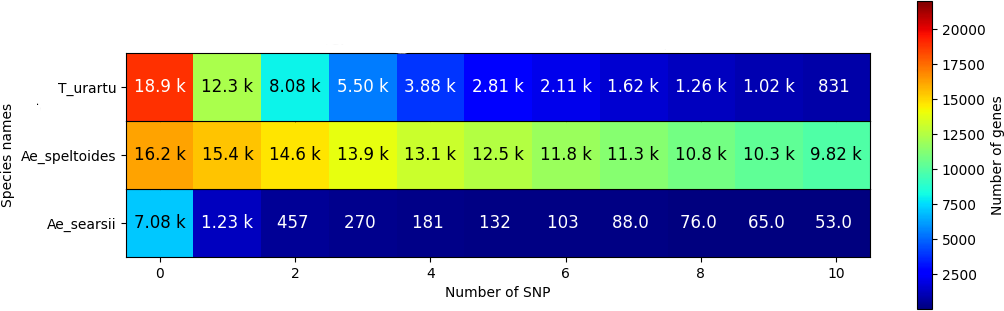
\includegraphics[width=0.95\textwidth]{Illustrations/Classic_results.png}
        \caption{Nombre de SNP par contig}
        \label{fig:heatmap_snp}
    \end{figure}

    \begin{alertblock}{Résultats}
        \begin{itemize}
            \small
            \item Besoin d'au moins 5 SNP par contig sur 70\% des contigs
            \item Seul 1 des 13 éspéces atteigne ce seuil
            \item Grande variabilité dans le npmbre de SNP (\textit{Aegilops searsii})
            \item \textit{Aegilops speltoides} candidat pour une étude préparatoire
        \end{itemize}
    \end{alertblock}

\end{frame}




\section{Re-Mapping}
\subsection{Justification}
\begin{frame}
	\tableofcontents[sectionstyle=show/shaded,subsectionstyle=show/show/hide,subsubsectionstyle=show/show/hide]
\end{frame}

\begin{frame}
    \begin{alertblock}{Explication des résultats précédents}
        \begin{itemize}
            \item Trop peux de reads ont mappés
            \item Le transcriptome été référence  de l'équipe est potentielment incomplet
        \end{itemize}
    \end{alertblock}

    \begin{alertblock}{Nouveaux mappings}
        \begin{itemize}
            \item Sur le génome de référence
            \item Sur le transcriptome de référence
            \item Sur l'ancien transcriptome de référence
        \end{itemize}
    \end{alertblock}

    \begin{alertblock}{Attendus}
        $Génome \geq transcriptome > Ancien_transcriptome$
    \end{alertblock}

\end{frame}

\subsection{Outils}

\begin{frame}{Outils }
   
        \begin{block}{GeCKO \cite{ardisson_gecko_2024}}
            \begin{itemize}
                \item Analyses de données NGS
                \item « user-friendly »
            \end{itemize}
        \end{block}


    \begin{block}{Mapper}
        \begin{itemize}
            \item Transcriptomes : BWA-MEM
            \item Génome : Minimap2
        \end{itemize}
    \end{block}

\end{frame}

\begin{frame}{Outils}
   
    \begin{block}{GeCKO \cite{ardisson_gecko_2024}}
        \begin{itemize}
            \item Analyses de données NGS
            \item « user-friendly »
        \end{itemize}
    \end{block}


    \begin{block}{Mapper}
        \begin{itemize}
            \item Transcriptomes : BWA-MEM
            \item Génome : Minimap2 \pause (Non-fonctionnel)
            \item Génome : STAR (Arrivé trop tard)
        \end{itemize}
    \end{block}
\end{frame}
% 
\subsection{Résultats}
\begin{frame}{Résultats}

    \begin{block}{Analyse}
        \begin{itemize}
            \item Nombre de reads par contigs
            \item Nombre de contigs ayants reçu des reads
            \item Qualité du mapping
        \end{itemize}
    \end{block}

    \pause
    \begin{itemize}
        \item[$\rightarrow$] \textbf{Le mapping sur l'ancien transcriptome est meilleur.}
    \end{itemize}





\end{frame}

% \begin{frame}{Résultats II}
%
%    \begin{figure}[ht]
%        \centering
%        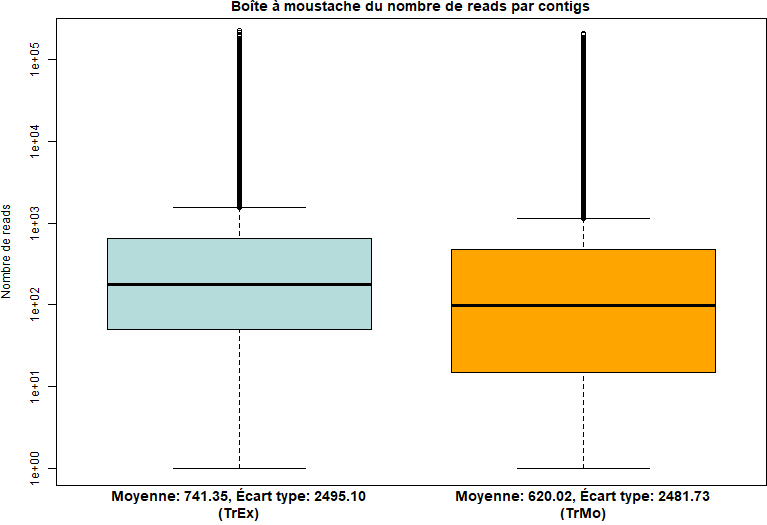
\includegraphics[width=0.9\textwidth]{./Illustrations/boxplotTr.png}
%        \caption{Boite }
%        \label{fig:BoxPlotContigs}
%    \end{figure}
%
% \end{frame}

\section{Conclusion}

\begin{frame}{Conclusion et Perspéctives}
    \begin{alertblock}{Conclusion}
        \begin{itemize}
            \item Le jeu de donné risque de ne pas convenir.
        \end{itemize}
    \end{alertblock}

    \pause

    \begin{exampleblock}{Perspéctives}
        \begin{itemize}
            \item Analyses du mapping sur le génome de référence
            \item La quantification des SNP n'a eu lieu que sur les "anciens BAM"
        \end{itemize}
    \end{exampleblock}
\end{frame}


\begin{frame}{Points clef}
    \begin{center}
        \huge \textbf{Merci pour votre attention}
    \end{center}

    \begin{block}{Points clefs de la présentation}
        \begin{itemize}
            \item Dévelopement d'un outil
            \item Quantification des SNP
            \item Remapping des BAMS
            \item Analyse des nouveaux BAM
        \end{itemize}
    \end{block}
       


\end{frame}


\appendix
\section*{annexes}
\begin{frame}
   \frametitle{Phylogénie}
   \subfile{annexes/phylogenetic-relationships}
\end{frame}

\begin{frame}{}
   \begin{figure}[ht]
      \centering
       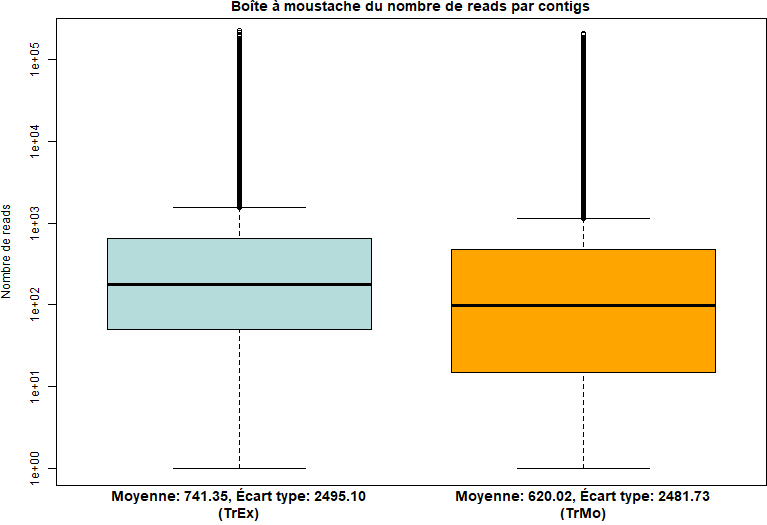
\includegraphics[width=0.9\textwidth]{./Illustrations/boxplotTr.png}
       \caption{Boite à moustache du nombre de reads par contigs}
       \label{fig:BoxPlotContigs}
   \end{figure}

\end{frame}

\begin{frame}[allowframebreaks]
   \frametitle{Références}
   \printbibliography
\end{frame}



\end{document}
